%==============================================================================
%== template for LATEX poster =================================================
%==============================================================================
%
%--A0 beamer slide-------------------------------------------------------------
\documentclass[final]{beamer}
\usepackage[orientation=portrait,size=a1, scale=1.1]{beamerposter}
\geometry{hmargin=2.5cm}
\usepackage[utf8]{inputenc}
\linespread{1.1}
\usepackage[export]{adjustbox}

\usetheme{ntnuposter} % Poster style


% Default plot settings
\pgfplotsset{legend style={fill=black!8!white,
                           at={(0.5,-0.25)},
                           anchor=north,
                           legend cell align=left,
                           legend columns=2,
                           column sep=0.3cm,
                           font=\footnotesize}}
\pgfplotsset{width=\textwidth, height=8cm}
\pgfplotsset{x tick label style={align=center}}
\pgfplotsset{every axis/.append style={font=\footnotesize}}
\pgfplotsset{every axis x label/.style={
    at={(0.5, -0.1)},
    anchor=north,
},}


\title[]{{\huge Gullfaks project} \\ \vspace{0.3em} {\large TPG4160 Reservoir Simulation}}
\subtitle{Gullfaks project}

\author{Einar Baumann \and Magnus Rodahl \and Yonas Haile}
\institute[]{Norwegian University of Science and Technology}
\date{\today}


\begin{document}
\begin{frame}[t]
%==============================================================================
\begin{multicols}{3}
%==============================================================================
%==The poster content==========================================================
%==============================================================================


% WBHP WGIR WGOR WGPT WGPR WOPT WOPR WPI1 WWCT
% A-1H A-2AH A-3H A-5H

% A-2AH A-3H A-8 A-10 A-11WAT A-12WAT A-13 A-14 A-17 A-1H A-5H A-35 A-38 A-39A B-37

% FGOR FGPR FGPT FOPR FOPT FWCT

\section{Introduction} % (fold)
The Gullfaks Field in the North sea consist of many reservoirs, and some of them are quite isolated from the rest. This makes them easier to simulate and for us to work on. We were assigned to work on Segment H1, which Statoil has developed an Eclipse reservoir model for



\section{Communication in the Lower Brent Group}
The Gullfaks H1 segment is an almost isolated part of the main Gullfaks field. It had an estimated STOOIP of $20,3 \,M\mathrm{Sm^3}$ oil and a recovery factor around 57\%. It is a part of the lower Brent Group,which is oil-filled part in the western and central parts of the Gullfaks structure. We see pretty good internal communication in this segment due to little internal faulting, and the formation is relatively homogenous.










\section{Base Case}
We made our base case model by stripping out everything but the 4 first wells  that are defined in the provided schedule file. The wells that remain are
\begin{itemize}
  \item Two producers: A-1H and A-2AH.
  \item An injector, A-5H.
\end{itemize}
Production data from this model is shown as a reference alongside data for other modified models on this poster.









\vskip7ex
\section{Impact of perforations}
Two modifications to the perforations in the wells were tested:
\begin{itemize}
  \item All \texttt{OPEN} sections were set to \texttt{SHUT}, and vice versa.
  \item All sections were set to open.
\end{itemize}
The results of both of these simulations are shown in Figure~\ref{fig:perfs_wopt_wwct}.

\begin{figure}[H]
  \centering
  \begin{tikzpicture}
  \begin{axis}[
      width=.75\columnwidth, height=10cm,
      title={A-1H well},
      xlabel=Days, ylabel=WOPT,
      xmin=0, ymin=0,
      xtick={0, 2000, 4000, 6000, 8000, 10000},
      axis y line* = left,
      legend entries={WOPT (original), WOPT(inverted), WOPT (all open), WWCT (original), WWCT(inverted), WWCT (all open)},
      ]
      \addlegendimage{ultra thick, blue}
      \addlegendimage{ultra thick, blue, dotted}
      \addlegendimage{ultra thick, blue, dashed}
      \addlegendimage{ultra thick, red}
      \addlegendimage{ultra thick, red, dotted}
      \addlegendimage{ultra thick, red, dashed}
    \addplot[ultra thick, color=blue] table[x=TIME, y=WOPT:A-1H, col sep=comma] {data/base.csv};
    \addplot[ultra thick, color=blue, dashed] table[x=TIME, y=WOPT:A-1H, col sep=comma] {data/changed_perforations_inverted.csv};
    \addplot[ultra thick, color=blue, dotted] table[x=TIME, y=WOPT:A-1H, col sep=comma] {data/changed_perforations_all_open.csv};
  \end{axis}
  \begin{axis}[
      width=.75\columnwidth, height=10cm,
      xlabel=Days, ylabel=WWCT,
      xmin=0, ymin=0,
      xtick={0, 2000, 4000, 6000, 8000, 10000},
      hide x axis,
      axis y line*=right,
      ]
    \addplot[ultra thick, color=red] table[x=TIME, y=WWCT:A-1H, col sep=comma] {data/base.csv};
    \addplot[ultra thick, color=red, dashed] table[x=TIME, y=WWCT:A-1H, col sep=comma] {data/changed_perforations_inverted.csv};
    \addplot[ultra thick, color=red, dotted] table[x=TIME, y=WWCT:A-1H, col sep=comma] {data/changed_perforations_all_open.csv};
  \end{axis}
\end{tikzpicture}

  \caption{}
  \label{fig:perfs_wopt_wwct}
\end{figure}

We see that both cases increase the water cut and reduce the oil production compared to the base model. This is due to layers with high $S_w$ be produced to a larger extent. In the case where the perforations are inverted, the reduced oil production rate can be explained by the perforations in the zones with high oil saturations being shut.

% Why do both altered cases have the same oil production?
% Why doesn't the water cut start rising earlier?







\section{Fault transmissibility}
Plots of the oil production rate for the two production wells in the base case model before and after setting the transmissibility across all faults to zero is shown Figure~\ref{fig:faults_opr}.

As expected, we see that the oil production rate drops to almost 0 after a relatively short time. This is because zero transmissibility across faults in a reservoir with many faults means that every well can only produce from a very small area around it.

In Figure~\ref{fig:faults_3d} we see one of the reasons why the production rate for the A-1H well is so much lower when the faults are closed. The large red area in the upper right part of the right image has very high $S_o$, even after producing for years. This is due to faults cutting the area off from the producing wells.


\begin{figure}[ht]
  \begin{tikzpicture}
  \begin{axis}[
      width=.75\columnwidth, height=10cm,
      title={},
      xlabel=Days, ylabel=WOPR,
      xmin=0, ymin=0,
      xtick={0, 2000, 4000, 6000, 8000, 10000, 12000, 14000},
      legend entries={A-1H (original), A-1H (closed faults), A-2AH (original), A-2AH (closed faults)},
      ]
      \addlegendimage{ultra thick, blue}
      \addlegendimage{ultra thick, blue, dashed}
      \addlegendimage{ultra thick, red}
      \addlegendimage{ultra thick, red, dashed}
    \addplot[ultra thick, color=blue] table[x=TIME, y=WOPR:A-1H, col sep=comma] {data/new_wells.csv};
    \addplot[ultra thick, color=blue, dashed] table[x=TIME, y=WOPR:A-1H, col sep=comma] {data/multflt_new_wells.csv};
    \addplot[ultra thick, color=red] table[x=TIME, y=WOPR:A-2AH, col sep=comma] {data/new_wells.csv};
    \addplot[ultra thick, color=red, dashed] table[x=TIME, y=WOPR:A-2AH, col sep=comma] {data/multflt_new_wells.csv};
  \end{axis}
\end{tikzpicture}

  \caption{}
  \label{fig:faults_opr}
\end{figure}


\begin{figure}[H]
  \begin{center}
    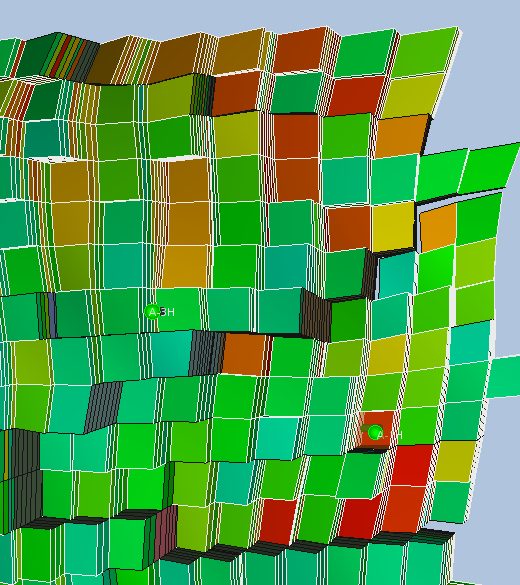
\includegraphics[clip=true, width=0.5\columnwidth, height=10cm]{images/soil_2010_base.png}
    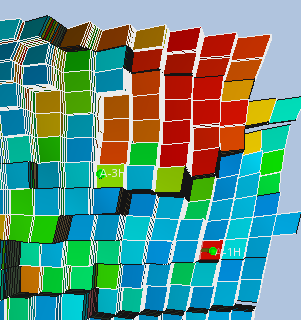
\includegraphics[clip=true, width=0.5\columnwidth, height=10cm]{images/soil_2010_multfl_0.png}
  \end{center}
  \caption{Oil saturation in 2010 in the same area for the base case (left) and the case with 0 transmissibility across faults (right).}
  \label{fig:faults_3d}
\end{figure}



\subsection{Net Present Value} % (fold)
\begin{center}
  $NPV_{\text{new wells}} - NPV_{\text{new wells, faults closed}}  = 643.9 \, \mathrm{MNOK}$
\end{center}



\end{multicols}
\end{frame}

\begin{frame}
\begin{multicols}{3}




\section{New wells}
New wells were placed using the following algorithm:
\begin{enumerate}
  \item Locate area with high oil saturation at final timestep. Place well there.
  \item If the well produces a reasonable amount of oil: leave it. If not: move it slightly. If the well is still not producing enough oil, remove it.
  \item Repeat 1. and 2. a few times.
\end{enumerate}
The results of placing three new wells, N-1, N-3 and N-4, are shown in Figures~\ref{fig:new_wells_wopt}, \ref{fig:new_wells_wopr} and \ref{fig:new_wells_field}.

We see that two of the three new wells (N-3 and N-4) produce approximately the same amount of oil as A-1H, while the last new well, N-1, produces significantly more. N-1 Also produces at a quite high rate for a long time.

From Figure~\ref{fig:new_wells_field} we see that the new wells lets us produce approximately twice the amount of oil compared to the base model.

\begin{figure}[H]
  \hspace{-5ex}\begin{tikzpicture}
  \begin{axis}[
      width=.75\columnwidth, height=10cm,
      title={},
      xlabel=Days, ylabel=WOPT,
      xmin=0, ymin=0,
      xtick={0, 2000, 4000, 6000, 8000, 10000, 12000, 14000},
      legend entries={A-1H, A-2AH, N-1, N-3, N-4},
      legend style={legend columns=5},
      ]
      \addlegendimage{ultra thick, blue}
      \addlegendimage{ultra thick, red}
      \addlegendimage{ultra thick, brown}
      \addlegendimage{ultra thick, green}
      \addlegendimage{ultra thick, orange}
    \addplot[ultra thick, color=blue] table[x=TIME, y=WOPT:A-1H, col sep=comma] {data/new_wells.csv};
    \addplot[ultra thick, color=red] table[x=TIME, y=WOPT:A-2AH, col sep=comma] {data/new_wells.csv};
    \addplot[ultra thick, color=brown] table[x=TIME, y=WOPT:N-1, col sep=comma] {data/new_wells.csv};
    \addplot[ultra thick, color=green] table[x=TIME, y=WOPT:N-3, col sep=comma] {data/new_wells.csv};
    \addplot[ultra thick, color=orange] table[x=TIME, y=WOPT:N-4, col sep=comma] {data/new_wells.csv};
  \end{axis}
\end{tikzpicture}

  \caption{}
  \label{fig:new_wells_wopt}
\end{figure}

\begin{figure}[H]
  \hspace{-5ex}\begin{tikzpicture}
  \begin{axis}[
      width=.75\columnwidth, height=10cm,
      title={},
      xlabel=Days, ylabel=WOPR,
      xmin=0, ymin=0,
      xtick={0, 2000, 4000, 6000, 8000, 10000, 12000, 14000},
      legend entries={A-1H, A-2AH, N-1, N-3, N-4},
      legend style={legend columns=5},
      ]
      \addlegendimage{ultra thick, blue}
      \addlegendimage{ultra thick, red}
      \addlegendimage{ultra thick, brown}
      \addlegendimage{ultra thick, green}
      \addlegendimage{ultra thick, orange}
    \addplot[ultra thick, color=blue] table[x=TIME, y=WOPR:A-1H, col sep=comma] {data/new_wells.csv};
    \addplot[ultra thick, color=red] table[x=TIME, y=WOPR:A-2AH, col sep=comma] {data/new_wells.csv};
    \addplot[ultra thick, color=brown] table[x=TIME, y=WOPR:N-1, col sep=comma] {data/new_wells.csv};
    \addplot[ultra thick, color=green] table[x=TIME, y=WOPR:N-3, col sep=comma] {data/new_wells.csv};
    \addplot[ultra thick, color=orange] table[x=TIME, y=WOPR:N-4, col sep=comma] {data/new_wells.csv};
  \end{axis}
\end{tikzpicture}

  \caption{}
  \label{fig:new_wells_wopr}
\end{figure}


\begin{figure}[H]
  \begin{tikzpicture}
  \begin{axis}[
      width=.75\columnwidth, height=10cm,
      xlabel=Days, ylabel=FOPR,
      xmin=0, ymin=0,
      xtick={0, 2000, 4000, 6000, 8000, 10000, 12000, 14000},
      axis y line* = left,
      legend entries={FOPR (new wells), FOPR (base), FOPT (new wells), FOPT (base)},
      ]
      \addlegendimage{blue}
      \addlegendimage{blue, dashed}
      \addlegendimage{red}
      \addlegendimage{red, dashed}
    \addplot[color=blue] table[x=TIME, y=FOPR, col sep=comma] {data/field_new_wells.csv};
    \addplot[color=blue, dashed] table[x=TIME, y=FOPR, col sep=comma] {data/field_base.csv};
  \end{axis}
  \begin{axis}[
      width=.75\columnwidth, height=10cm,
      xlabel=Days, ylabel=FOPT,
      xmin=0, ymin=0,
      xtick={0, 2000, 4000, 6000, 8000, 10000, 12000, 14000},
      hide x axis,
      axis y line*=right,
      ]
    \addplot[color=red] table[x=TIME, y=FOPT, col sep=comma] {data/field_new_wells.csv};
    \addplot[color=red, dashed] table[x=TIME, y=FOPT, col sep=comma] {data/field_base.csv};
  \end{axis}
\end{tikzpicture}

  \caption{}
  \label{fig:new_wells_field}
\end{figure}


\subsection{Net Present Value} % (fold)

\begin{center}
  $NPV_{N-1} = 516.7 \, \mathrm{MNOK}$

  $NPV_{N-3} = 490.5 \, \mathrm{MNOK}$

  $NPV_{N-4} = 582.2 \, \mathrm{MNOK}$
\end{center}









\section{Injection of Abio Gel} % (fold)

\subsection{Mechanisms} % (fold)
\emph{Abio Gel} consists mainly of sodium silicate. When it comes into contact with divalent cations (e.g. calcium and magnesium) -- found in seawater and in the formation -- it reacts, forming a stiff gel if the concentration of cations is sufficiently high.

When it is injected into the reservoir it reduces the permeability in the invaded areas, thus forcing the water to find new, less paths. This lets us hit bypassed oil which may now be forced towards producers. This is illustraded in Figure~\ref{fig:abio_gel}.

\begin{figure}[H]
  \centering
  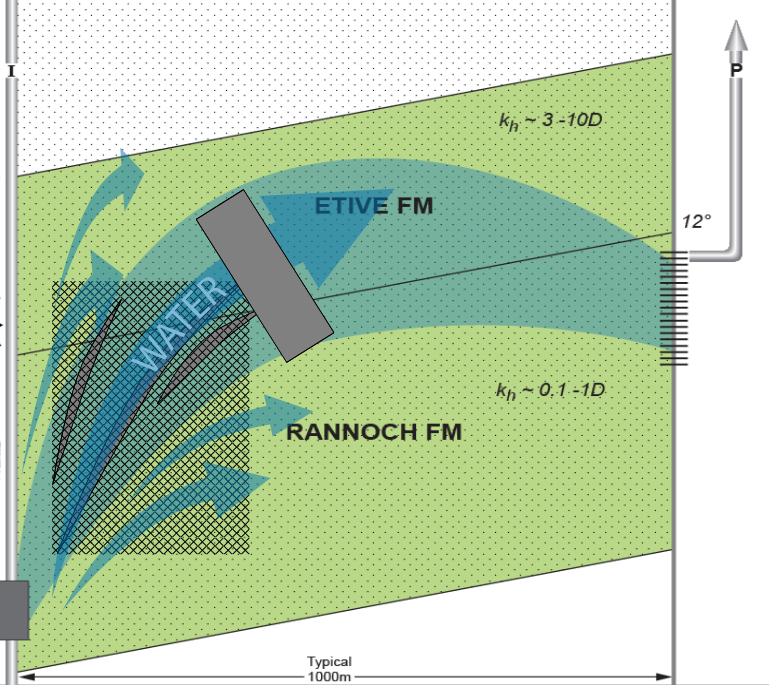
\includegraphics[width=0.5\columnwidth]{images/abio_gel.png}
  \caption{}
  \label{fig:abio_gel}
\end{figure}


\vskip5ex
\subsection{Eclipse representation} % (fold)
To get the effects of the Abio Gel in the Eclipse model we used a tracer. The property calculator in FloViz was then used to create a new property equal to some fraction of the permeability, dependent on the amount of tracer found in the blocks. Blocks with a large amount of tracer had the property set to a small fraction, blocks with no tracer were left unaltered. This values of this new property was then applied as permeability in the simulation grid. The resulting altered permeability is shown in Figure~\ref{fig:abio_area}.




% Bildene er fra 2. juni 2012
% Kun blokker med EORF > 1 er vist
% Injisert med A-35

\begin{figure}[H]
  \centering
  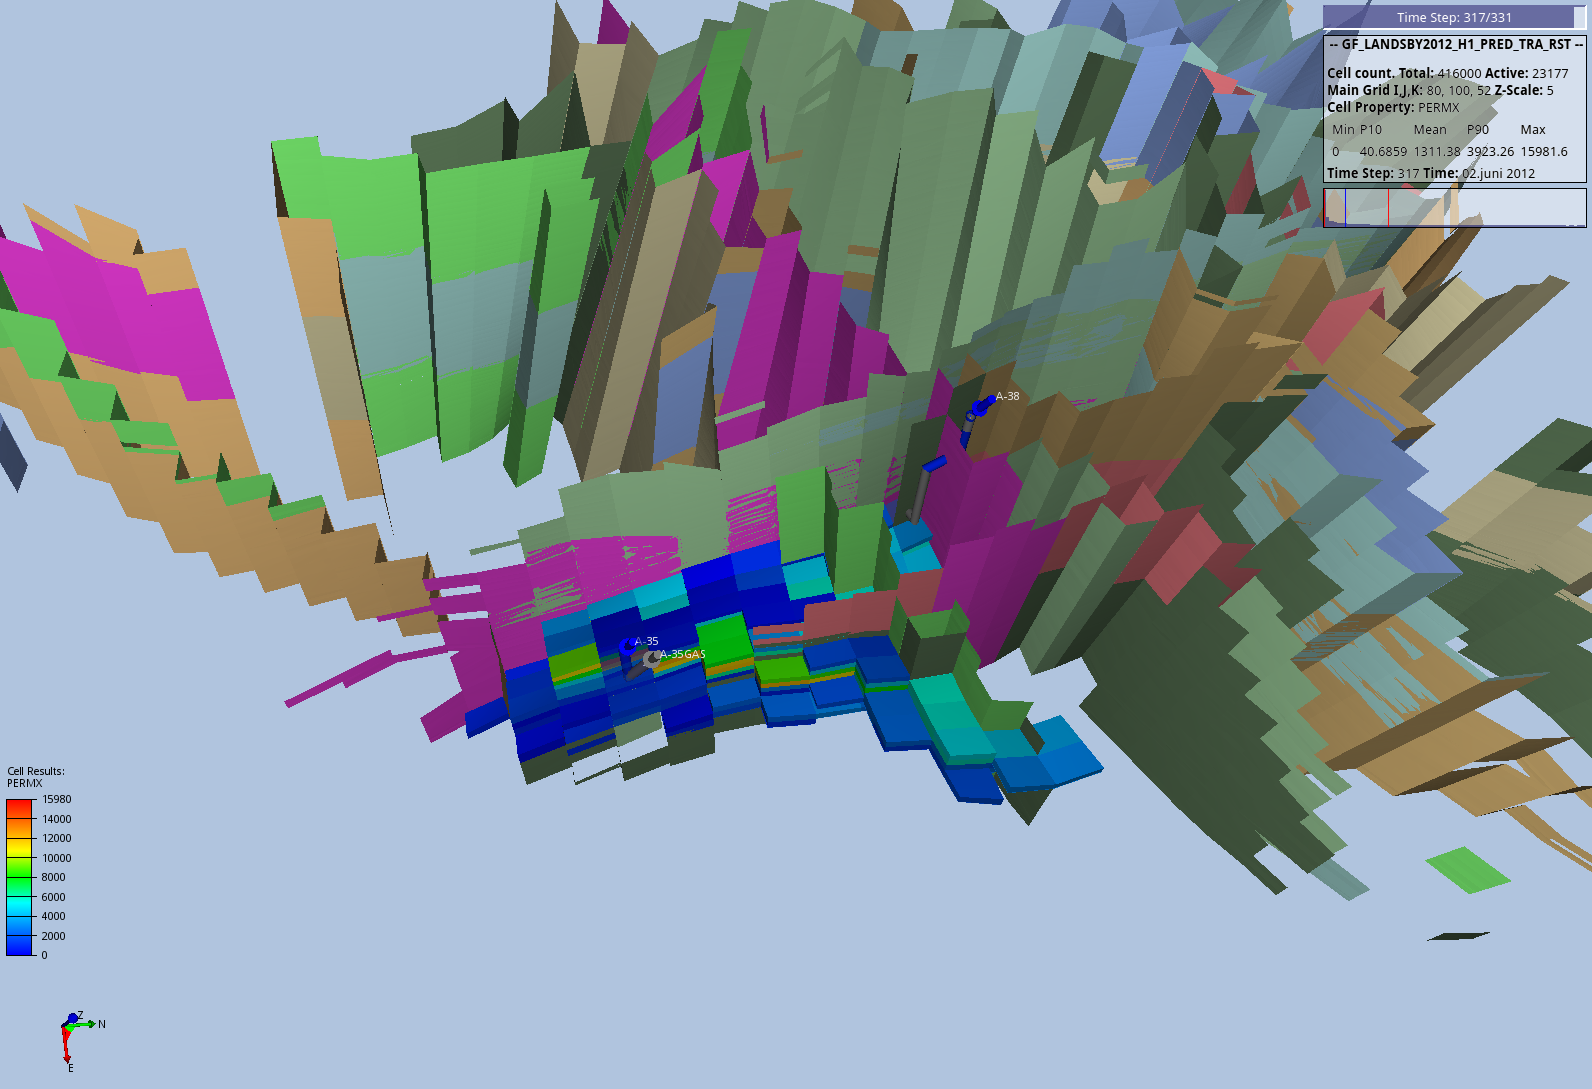
\includegraphics[clip=true, trim=12cm 7cm 13cm 13cm, width=0.5\columnwidth]{images/before_permedit.png}
  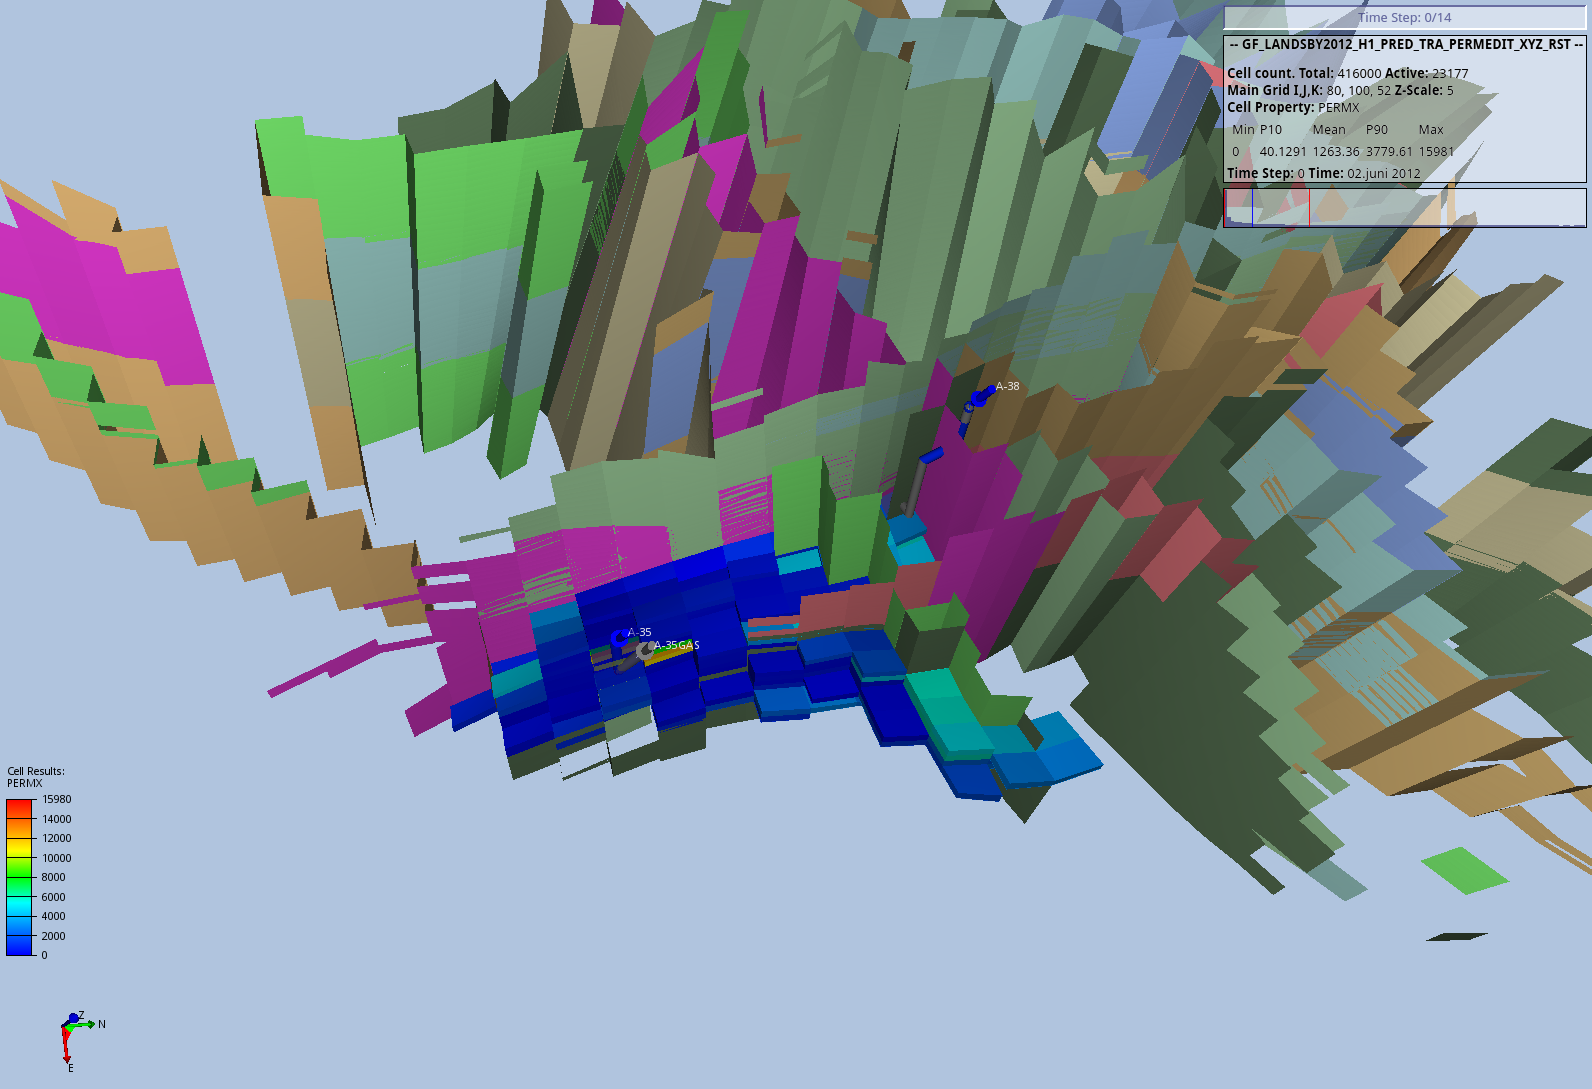
\includegraphics[clip=true, trim=12cm 7cm 13cm 13cm, width=0.5\columnwidth]{images/after_permedit.png}
  \caption{Area affected by the tracer, color mapped according to permeability (blue is lowest) before (left) and after (right) changing the permeability.}
  \label{fig:abio_area}
\end{figure}

\subsection{Results after injection} % (fold)
Figure~\ref{fig:abio_change} shows that injecting the Abio gel significantly increases production from the A-39A well compared to the original model.

\begin{figure}[H]
  \centering
  \begin{tikzpicture}
  \begin{axis}[
      width=.75\columnwidth, height=10cm,
      title={A-39A},
      xlabel=Days, ylabel=WOPR,
      xmin=0, ymin=0,
      xtick={0, 2000, 4000, 6000, 8000, 10000 ,12000, 14000},
      axis y line* = left,
      legend entries={WOPR before, WOPR after, WOPT before, WOPT after},
      ]
      \addlegendimage{red, dashed}
      \addlegendimage{red}
      \addlegendimage{blue, dashed}
      \addlegendimage{blue}
    \addplot[ultra thick, red, dashed] table[x=TIME, y=WOPR:A-39A, col sep=comma] {data/before_permedit.csv};
    \addplot[ultra thick, red] table[x=TIME, y=WOPR:A-39A, col sep=comma] {data/after_permedit.csv};
  \end{axis}
  \begin{axis}[
      width=.75\columnwidth, height=10cm,
      xlabel=Days, ylabel=WOPT,
      xmin=0, ymin=0,
      xtick={0, 2000, 4000, 6000, 8000, 10000},
      hide x axis,
      axis y line*=right,
      ]
    \addplot[ultra thick, blue, dashed] table[x=TIME, y=WOPT:A-39A, col sep=comma] {data/before_permedit.csv};
    \addplot[ultra thick, blue] table[x=TIME, y=WOPT:A-39A, col sep=comma] {data/after_permedit.csv};
  \end{axis}
\end{tikzpicture}



  \caption{Production from the A-39A well before and after injection of Abio gel.}
  \label{fig:abio_change}
\end{figure}

\subsection{Net Present Value}
\begin{center}
  $NPV_{Abio} = 206.5 \, \mathrm{MNOK}$
\end{center}


%==============================================================================
%==End of content==============================================================
%==============================================================================


\end{multicols}

%==============================================================================
\end{frame}
\end{document}
